\section{Celda Universal}

\subsection{Configuraciones de celdas}

\subsubsection{Kerwin-Huelsman-Newcomb}

\begin{figure}[H] %!ht
	\centering
	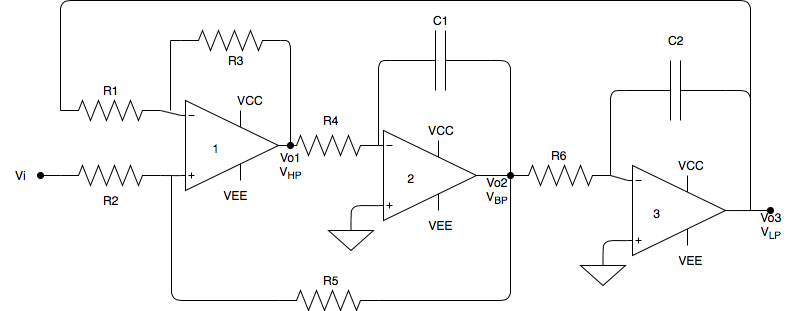
\includegraphics[width=10cm,height=10cm,keepaspectratio]{../EJ4/kerwin.png}
	\caption{Circuito Kerwin-Huelsman-Newcomb}
	\label{kerwin}
\end{figure}

\subsubsection{Tow-Thomas}

\begin{figure}[H] %!ht
	\centering
	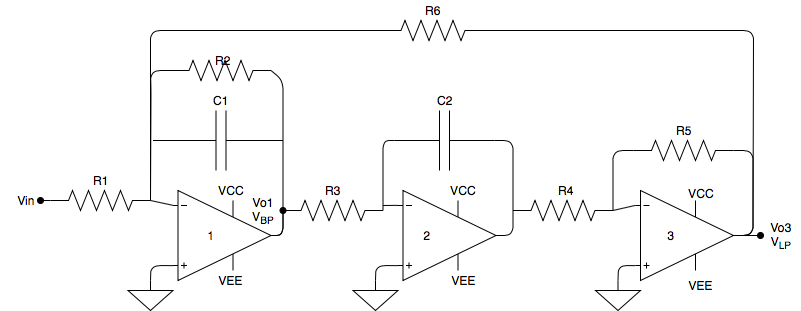
\includegraphics[width=10cm,height=10cm,keepaspectratio]{../EJ4/tow_thomas.png}
	\caption{Celda Tow-Thomas}
	\label{tow_thomas}
\end{figure}

\subsubsection{Ackerberg-Mossberg}

\begin{figure}[H] %!ht
	\centering
	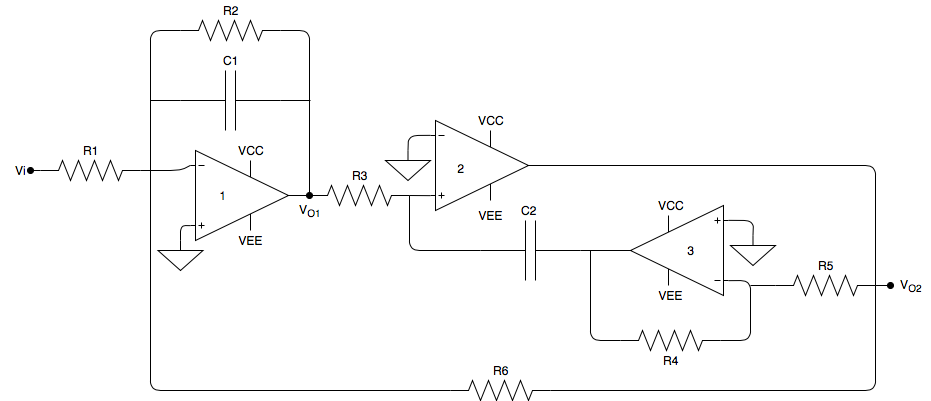
\includegraphics[width=10cm,height=10cm,keepaspectratio]{../EJ4/ackerberg.png}
	\caption{Celda Ackerberg-Mossberg}
	\label{ackerberg}
\end{figure}

\subsubsection{Fleischer-Tow}

\begin{figure}[H] %!ht
	\centering
	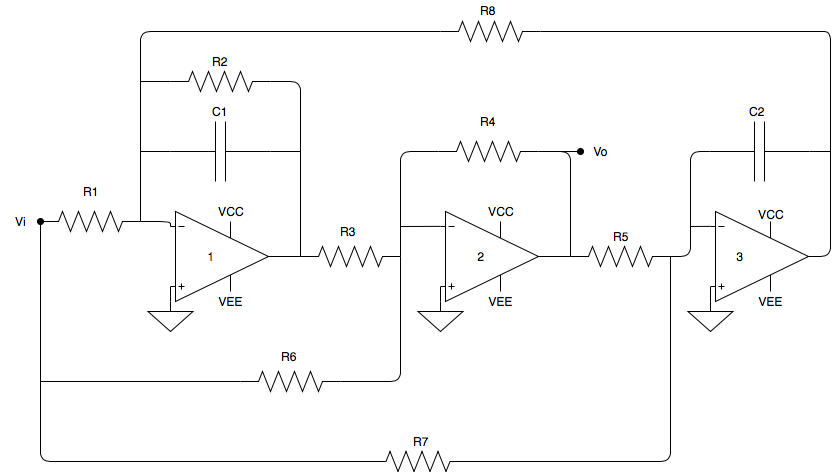
\includegraphics[width=10cm,height=10cm,keepaspectratio]{../EJ4/fleischer.png}
	\caption{Celda Fleischer-Tow}
	\label{fleischer}
\end{figure}